%  Created by Branden Stone on 2015-01-15.
%  Copyright (c) 2015 Branden Stone. All rights reserved.
%--------------------------------------------------------
\documentclass{article}


%---------------------------
% Packages
%---------------------------
\usepackage{amssymb, amsmath, latexsym, amsfonts, amsthm, mathrsfs} % Standard packages that are nice to have.
\usepackage{amsrefs} % Allows for easy referencing and citations.
\usepackage{verbatim} % Needed for \begin{comment} \end{comment}.
\usepackage[text={6in,9in},centering]{geometry} % Defines the dimensions of the text body.
\usepackage[colorlinks=true]{hyperref} % Allows for use of hyperlinks.
%\usepackage[doublespacing]{setspace} % Makes the document double spaced.
\usepackage[pdftex]{graphicx} % Allows for \includegraphics
\usepackage{enumerate} % Allows for easy modification of lists

\renewcommand{\arraystretch}{1.5}

%----------------------------
% Title and Author
%----------------------------

\title{Math 390: Practice Problems for Quiz 2}
\author{}
\date{}


%----------------------------
% Main Document Body
%----------------------------

\begin{document}


%-------------------------------------------------------------
% Front Matter: This is where you can add a table of contents,
% preface, list of figures, ETC. for this template we will 
% only create a title and author name with `\maketitle'
%-------------------------------------------------------------

\maketitle

\setlength{\parindent}{0em} % Sets indentation of new paragraph
\setlength{\parskip}{1em} % Sets space between paragraphs

%-------------------------------------------------------------
% Document Body: Essentially this is where you place the 
% content of your document. To use this template, just delete
% all of the text between here and the Bibliography Section.
% Then type whatever you desire.
%-------------------------------------------------------------

\section*{Problems from the book}
\begin{center}
\begin{tabular}{lll}
	\underline{$4^{\text{th}}$ Edition} & & \underline{$5^{\text{th}}$ Edition} \\
	{ \it Section 17:} 17.1, 17.3 & & { \it Section 5.1:} 5.1, 5.3 \\
	{ \it Section 21:} 21.1, 21.2(i) & & { \it Section 5.2:} 5.9, 5.11(i) \\
	{ \it Section 29:} 29.4 & & { \it Section 6.3:} 6.21
\end{tabular}
\end{center}

\section*{Additional Problems}

\begin{enumerate}
	\item For each of the following graphs, compute the chromatic number $\chi(G)$ of the graph, and show a coloring that uses the minimum number of colors.
	\begin{center}
	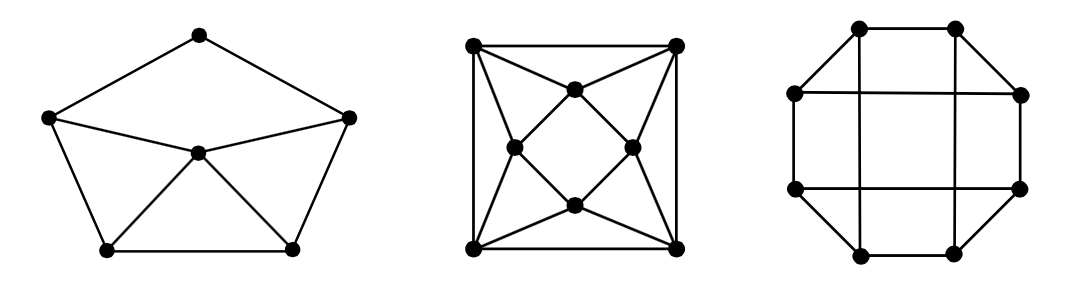
\includegraphics[width=.6\textwidth]{pic1.png}
	\end{center}

	\item For each of the following graphs, compute the chromatic index $\chi'(G)$ of the graph, and show an edge-coloring that uses the minimum number of colors.
	\begin{center}
	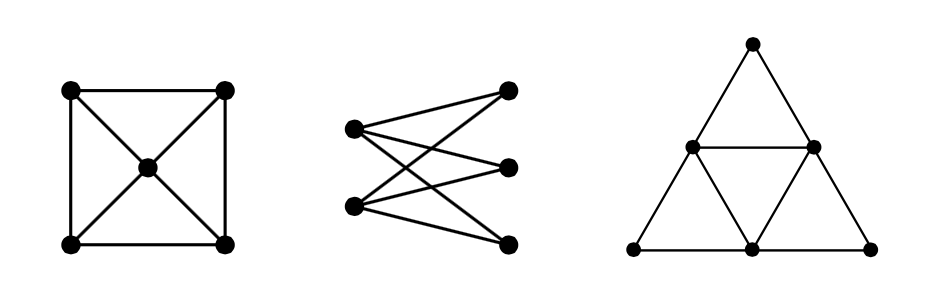
\includegraphics[width=.6\textwidth]{pic2.png}
	\end{center}

	\item For each of the following graphs, compute the chromatic polynomial $P_G(k)$.
	\begin{center}
	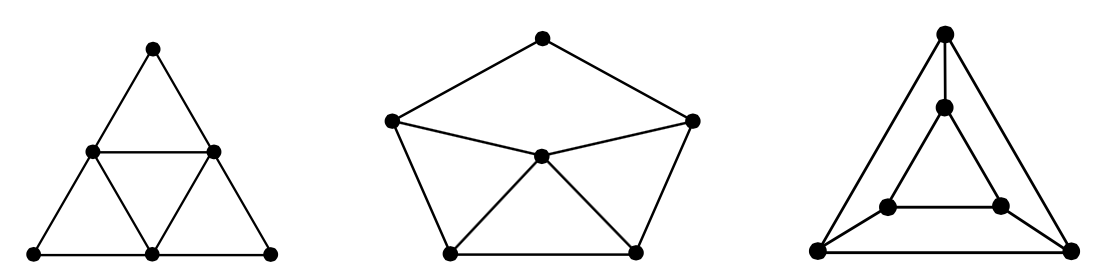
\includegraphics[width=.6\textwidth]{pic3.png}
	\end{center}	

\pagebreak

	\item Consider the following Markov chains:
	\begin{center}
	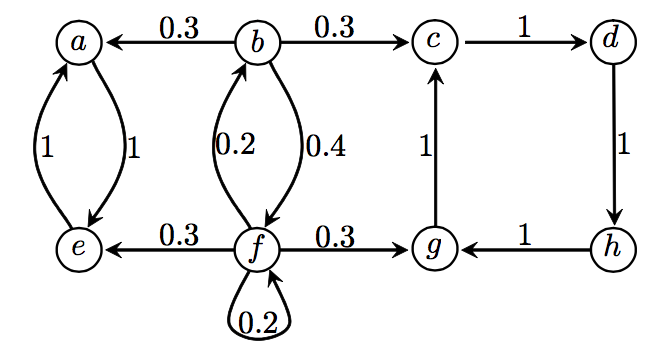
\includegraphics[width=.5\textwidth]{pic4.png}
	\end{center}

	\begin{enumerate}
		\item Which states in the Markov chain are persistent? Which states are transient?

		\item For each state of the Markov chain, determine whether the state is periodic. If it is periodic, what is its period?

		\item Is the Markov chain ergodic?
	\end{enumerate}

	\item Consider the following Markov chains:
	\begin{center}
	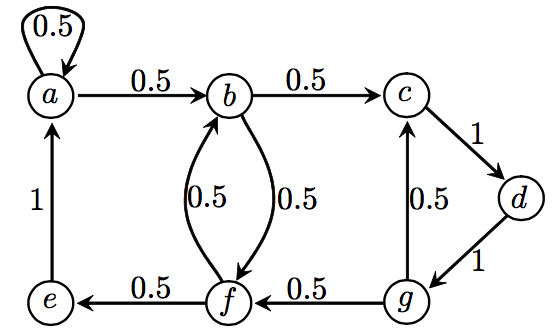
\includegraphics[width=.5\textwidth]{pic5.png}
	\end{center}	


	\begin{enumerate}
		\item Which states in the Markov chain are persistent? Which states are transient?

		\item For each state of the Markov chain, determine whether the state is periodic. If it is periodic, what is its period?

		\item Is the Markov chain ergodic?
	\end{enumerate}

	\item There are two competing cellphone companies in a city, Company A and Company B. In 2015, 40\% of the people in the city use Company A, and 60\% of the people use Company B. Each year 40\% of the people who who use Company A switch to using Company B, and 30\% of the people who use Company B switch to using Company A. (Assume that everyone in the city has a cellphone with either Company A or Company B.)

	\begin{enumerate}
		\item Model this situation with a Markov chain. Find the transition matrix and associated digraph that describes the number of people using each company.

		\item What percent of people will use Company A in 2016?

		\item Assuming the trend continues, what fraction of people will use Company A in the long run?
	\end{enumerate}

\pagebreak

	\item Consider the following network:
	\begin{center}
	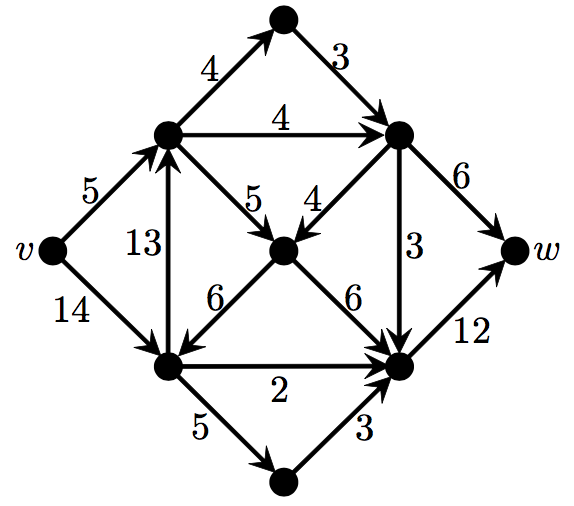
\includegraphics[width=.4\textwidth]{pic6.png}
	\end{center}	

	\begin{enumerate}
		\item Find a maximum flow in the above network.
		\item Fine a minimum cut in the above network.
	\end{enumerate}




	


\end{enumerate}


\end{document}